\begin{fact} \label{ln-tab-var}
	La fonction $\ln$ admet le tableau de variations suivant.
	%
	\begin{center}
        \begin{tikzpicture}
            \tkzTabInit{
            	$x$      / 1 , 
				$\ln x$  / 1.5
			}{$0$, $+\infty$}

            \tkzTabVar{D-/ {\small$-\infty$}, +/ {\small$+\infty$}}
        \end{tikzpicture}
	\end{center}
\end{fact}


\begin{proof}
	La monotonie est donnée par le fait \reffact{ln-mono}.
	Le calcul des limites se fait à la main sans souci, en notant au préalable que, par stricte croissance, $\ln 10 > \ln 1$ donne $\ln 10 > 0$.
	%
	\begin{itemize}
		\item Soit $A \in \RR$.
		Il existe $n \in \NN$ tel que $n \ln 10 > A$.
		Or, pour $x > 10^n$, nous avons $\ln x > \ln(10^n)$, puis $\ln x > A$, via $\ln(10^n) = n \ln 10$.
		%
		En résumé,
		$\forall A \in \RR$, $\exists x_0 \in \RRsp$ tel que $x > x_0$ implique $\ln x > A$.
		Ceci est la définition de $\limit{\ln x}{x}{+ \infty} = +\infty$.
		
		\item Pour la limite en $0^+$, le plus efficace est de passer via $\ln(\frac1x) = - \ln x$ qui donne
		$\limit{\ln x}{x}{0^+} = - \limit{\ln x}{x}{+ \infty}$.
		%
		On peut aussi le faire à la main via $10^{-n}$.
	\end{itemize}
	
	\null
	\vspace{-6ex}
\end{proof}

\vspace{1ex}
